%% LaTeX_Thesis_Template.tex
% An unofficial LaTeX template for Cranfield theses.
% 2017/08/14 Daniel Auger's unofficial Cranfield thesis .sty file
% 2023/05/31 Updated by Shaun Forth (SAF) for logo inclusion
% 2023/06/08 SAF removed capitalisation on title pages on advice of Amy 
% Greenaway and Alison Waters. Added Daniel Auger's headers with 
% chapter and section names.
% 2023/06/08 SAF simplified logo inclusion

%%
% This document is an example of the use of the unofficial "cranfieldthesis" 
% LaTeX style file.  I hope it's useful, and a good likeness of the Word template.

\documentclass[12pt,oneside]{book} % for one-sided printing
%\documentclass[12pt,twoside]{book} % for two-sided printing


% Use the custom "cranfieldthesis" LaTeX style file. 
\usepackage{cranfieldthesis}
\usepackage{lscape} % for landscape pages
\usepackage{amsmath}
\usepackage{enumitem}
\usepackage{changepage}
\usepackage{pdfpages}
\usepackage{blindtext}% Just used so we can generate some example text
\usepackage{algorithm}
\usepackage{algpseudocode}
\usepackage{amssymb}
\usepackage{mathtools}
\usepackage[export]{adjustbox}
\usepackage{lipsum}
\usepackage{booktabs}  % For better quality tables
\usepackage{siunitx}
\usepackage{float}
\usepackage{longtable} % Pour les tableaux sur plusieurs pages
\usepackage{tabularx}  % for the X column type
\usepackage{listings}
\usepackage{xcolor}
\usepackage{caption}
\usepackage{xfrac}
\usepackage{indentfirst}
\usepackage{subcaption}
\usepackage{graphicx}
\usepackage{geometry}
\usepackage{titlesec}
\geometry{a4paper, margin=1in}
\hypersetup{
    colorlinks,
    linkcolor={blue!50!blue},
    citecolor={blue!50!blue},
    urlcolor={blue!80!blue}
}

% By default, LaTeX uses a serif font - these are traditionally thought to be
% easier to read.   If you'd prefer sans-serif, please uncomment the 
% following line.
% \renewcommand{\familydefault}{\sfdefault}


% Example parameters for a typical taught MSc course
\title{Future Position Prediction for Pressure Refuelling Port
of Commercial Aircraft}
\author{Alexis Balayre}
\date{May 2024}
\school{\SATM}
\course{Computational and Software Techniques in Engineering}
\degree{MSc}
\academicyear{2023 - 2024}
% \setCUTextLogo % uncomment to set CU as text on title pages
\setCUPartnerLogo{logo-airbus.png} % uncomment to set joint CU and Partner logos on title 
% pages where PartnerLogo.[png,jpg,pdf,...] is the graphics file for the Partner Logo
%
% Supervisors
% Single supervisor - Use below 
%
%\supervisor{Dr First A. Supervisor}
%
% Multiple Supervisors,  use \supervisers. 
\supervisors{Dr Boyu Kuang and Dr Stuart Barnes}
% Associate supervisor use
%\associatesupervisor{Dr Associate Supervisor}
% Multiple associate supervisor use
%\associatesupervisors{Dr Associate Supervisor and Prof. Yet Another}

\copyrightyear{2024}

%	% Example parameters for a typical PhD
%	\title{My Thesis Title}
%	\author{A.\ Student}
%	\date{August 2014}
%	\school{School of Aerospace, Transport and Manufacturing}
%	\course{Transport Systems}
%	\degree{PhD}
%	\academicyear{2016--2017}
%       \supervisortext{Supervisors}  % changes from "Supervisor" to "Supervisors"
%	\supervisor{Dr D.\ J.\ Auger, Dr A.\ N.\ Other}
%	\copyrightyear{2017}
%	\fulfilment{} % removes message about partial fulfilment

%% COPYRIGHT NOTICES
%
% By default, a Cranfield University copyright statement is displayed. 
% MOD sponsored student theses will usually be Crown Copyright, and 
% should use the following command:
%
%	\copyrightholder{Crown Copyright}
%
% Do something similar if your copyright belongs to anyone else

% References
% Cranfield Numbered Style
\usepackage[numbers]{natbib} % for nice referencing
 \makeatletter % Reference list option change to number and period
 \renewcommand\@biblabel[1]{#1.} % from [1] to 1
 \makeatother %
 \setcitestyle{round} % use round citations
 
\begin{document}

%% Front matter
%
% This is where we do the title page, etc.
%

\frontmatter

% Standard-Form Title Pages
\maketitle
    
% Abstract and Keywords
\begin{abstract}
Replace with your abstract text of not more than 300 words.
\end{abstract}

\begin{keywords}
Replace with at least 6, semicolon seperated keywords (not contained within the thesis title) – this makes the thesis searchable.
\end{keywords}

% Acknowledgements
\chapter{Acknowledgements}
The author would like to thank \dots

% Use single spacing for Table of Contents, List of Figures, etc
{
\clearpage
\singlespacing
% Table of Contents
{
\tableofcontents
}
\clearpage

% List of Figures
\listoffigures

\clearpage
% List of Tables
\listoftables
}

% The list of abbreviations can't be automatically generated so you need to populate it yourself
\begin{listofabbreviations}
    \abbrev{SATM}{School of Aerospace, Technology and Manufacturing}
    \abbrev{SEEA}{School of Energy, Environment and Agrifoods}
    \abbrev{CDS}{Cranfield Defence and Security}
\end{listofabbreviations}





%% Main Matter
%
% This is where we include the main thesis content.
%
\mainmatter
\pagestyle{fancy}
\fancyhead[L]{\nouppercase{\leftmark}}
\fancyhead[R]{\nouppercase{\rightmark}}
%\fancyhead[L]{\thetitle}
%\fancyhead[C]{}
%\fancyhead[R]{\theauthor}
%\fancyfoot[L]{}
%\fancyfoot[C]{\thepage}
%\fancyfoot[R]{}

\chapter{Guidance}
\label{chap:Guidance}
For Chapter Titles use \verb#\chapter{chapter title}# and add an optional\linebreak \verb#\label{label name}# for easy cross referencing. 

\section{The Title Pages}
\label{sec:TitlePages}
The two title pages and the {\em Academic Integrity Declaration} are created using the \linebreak\verb#maketitle# command.  However, information for the title pages is set in the preamble (before \verb#\make{document}#) using various commands. Title, author and date are set  using the standard \LaTeX\ commands \verb#\title#, \verb#\author# and \verb#\date#. Other commands are included by \verb#cranfieldthesis.sty# as we now detail.

\subsection{Supervisors}
\label{sec:Supervisor}
If there is a single superviors (plus one or more associate superviors - see \refsec{sec:AssociateSupervisor}) then use \verb#\supervisor#,
\begin{verbatim}
\supervisor{Dr First A. Supervisor}
\end{verbatim}
But, if there are two or more then use \verb#\supervisors# with appropriate use of {\tt and}, commas, or \verb#\\# (for a line break)  to separate them,
\begin{verbatim}
\supervisors{Dr First A. Supervisor and Prof Second Supervisor}
\end{verbatim}
or,
\begin{verbatim}
\supervisors{Dr First A. Supervisor, Prof Second Supervisor\\ 
and Third Supervisor}
\end{verbatim}
You must set either the supervisor or supervisors. 

\subsection{Associate Supervisors}
\label{sec:AssociateSupervisor}
If there is a single associate supervior then use \verb#\associatesupervisor#,
\begin{verbatim}
\associatesupervisor{Dr Associate Supervisor}
\end{verbatim}
But, if there are two or more then use \verb#\associatesupervisors# with appropriate use of {\tt and}, commas, or \verb#\\# (for a line break)  to separate them,
\begin{verbatim}
\associatesupervisors{Dr Associate Supervisor and Prof. Yet Another}
\end{verbatim}
If you do not set the associate supervisor(s) then nothing is displayed.

\subsection{School, Course, Degree and Academic Year}
\label{sec:SchoolCourse}
Additional information on which Cranfield School of study and which course was undertaken are which degree is being sought are set using \verb#\school#, \verb#course#, \verb#degree# and \verb#\academicyear#.

\subsubsection{School}
\label{sec:School} 
Use command \verb#\school# to set your Cranfield School of study. There are predefined commands for each of our 4 schools. So you might use
\begin{verbatim}
\school{\CDS}
\end{verbatim}
for \CDS. Other schools may be specified using \verb#\SATM#, \verb#\SOM# or \verb#\SWEE#.

\subsubsection{Course}
\label{sec:Course}
Use command \verb#\course# to set your course title. e.g.,
\begin{verbatim}
\course{Military Operational Research}
\end{verbatim}
If this command is not set then no course title is written.

\subsubsection{Degree}
\label{sec:degree}
Command \verb#\degree# is used to set your degree of study. 

For taught programmes \cite{cranfield_university_taught_2023} this should be one of 
\begin{itemize}
\item MSc
\item MBA
\item MTech
\item MRes
\item MDes
\item PgDip
\item PgCert
\end{itemize}
For research programmes \cite{cranfield_university_research_2023} this should be one of 
\begin{itemize}
\item PhD
\item Executive DBA
\item EngD
\item MPhil
\item MSc by Research
\end{itemize}
For example,
\begin{verbatim}
\degree{MSc}
\end{verbatim}

\subsubsection{Academic Year}
\label{sec:AcademicYear}
Aside from the usual \verb#\date# which should be used to supply the month and year of your thesis submission, your should also use \verb#\academicyear# to supply the academic year. For example,
\begin{verbatim} 
\academicyear{2022--2023}
\end{verbatim}

\subsection{Copyright}
\label{sec:copyright}
The copyright year must be supplied, this will be the same as the year of submission. For example,
\begin{verbatim} 
\copyrightyear{2023}
\end{verbatim}
By default, a Cranfield University copyright statement is displayed. MOD sponsored student theses will usually be Crown Copyright, and should use the following command:
\begin{verbatim}
\copyrightholder{Crown Copyright}
\end{verbatim}
Do something similar if your copyright belongs to anyone else.

\subsection{Fulfilment}
\label{sec:Fulfilment}
By default the statement,
\begin{quote} 
This thesis is submitted in partial fulfilment of the requirements for the degree of ...
\end{quote}
is added to the second title page. This should be removed for degrees assessed entirely by the thesis, such as a PhD, by using the command,
\begin{verbatim}
\fullfillment{}
\end{verbatim}
in the preamble. 

\section{Section Heading}
\label{sec:SectionHeading}
For section headings use \verb#\section{section name}# and add an optional \linebreak\verb#\label{label name}# for easy cross referencing. 

\subsection{Subsection heading}
\label{sec:SubsectionHeading}
For subsection headings use \verb#\section{subsection name}# and add an optional \linebreak\verb#\label{label name}# for easy cross referencing. 

\subsubsection{Referring to headings}
Avoid referring to other parts of your document using phases such as ``{\em as described below}'' (unless on the same page, this could be anywhere in the rest of the thesis) or ``{\em as described previously}''  (this could be anywhere from the start of the thesis). Instead make use of the chapter and section labels to point the reader directly to the appropriate part of the thesis. 

Command \verb#\refchap{label name}# has been defined to make it easy to cross-refer\-ence chapters. Similarly, \verb#\refsec{label name}# is used to cross-reference section, subsection and subsubsection numbers. These commands should be used  when the cross-reference occurs mid-sentence to facilitate their abbreviation. For example, to produce
\begin{quote}
In \refchap{chap:Guidance} we provide guidance on formatting your thesis including, in \refsec{sec:SectionHeading}, section headings. 
\end{quote}
use:
\begin{verbatim}
In \refchap{chap:Guidance} we provide guidance on formatting your 
thesis including, in \refsec{sec:SectionHeading}, section headings. 
\end{verbatim}

At the start of sentences use commands \verb#\refChap{label name}# and\linebreak \verb#\refSec{label name}# to ensure abbreviations for Chapter and Section are not used. For example,
\begin{quote}
\refChap{chap:Guidance} provides guidance on formatting your thesis
including. \refSec{sec:SectionHeading} covers section headings. 
\end{quote}
is produced using
\begin{verbatim}
\refChap{chap:Guidance} provides guidance on formatting your thesis
including. \refSec{sec:SectionHeading} covers section headings. 
\end{verbatim}
At the time of writing, \verb#\refChap# and \verb#\refchap# produce the same output, but both are included for completeness and in case guidance changes in the future.

\section{Chapter and Section Page Breaks}
Use of the \verb#\chapter# command will automatically start a new page. Use of \verb#\section#, \verb#\subsection#  and \verb#\subsubsection# will not. If a page break is desired for improved formatting (e.g. a section title appears as the last line on a page and its text appears on the next), then use \verb#\pagebreak# to force a new page where you need it.  


\section{The Cranfield University logo and co-branding}
It is preferred that the Cranfield University logo is positioned at the top of the cover and title pages of the thesis document. The logo image files is provided as \verb#CULogo.png# with this template and included by default. (It can also be specified using the command \verb#\setCULogo#.)

If it is not appropriate to show the Cranfield University logo, then it can be removed and replaced by the text as described in \refsec{sec:UseCUText}.

If you are working with a partner on the research included in this thesis document, you may, subject to their approval, also include their official logo as co-branding on the cover and title pages. Guidance is provided in \refsec{sec:UsePartnerLogo}.



\subsection{Using Cranfield University text in place of a logo}
\label{sec:UseCUText}
If appropriate you may remove the Cranfield University logo from the cover and title pages of the thesis and in its place use the text “CRANFIELD UNIVERSITY”.

To remove the Cranfield logo issue the command
\begin{verbatim}
\setCUTextLogo
\end{verbatim}

\subsection{Adding a partner logo}
\label{sec:UsePartnerLogo}
Before using a partner logo in this document you must:
\begin{itemize}
\item obtain permission from the partner to use their logo in this document.
\item obtain a high-resolution logo from the organisation – do not take a screen-shot from the website.
\end{itemize}
To add the partner logo as co-branding use
\begin{verbatim}
\setCUPartnerLogo{PartnerLogo}
\end{verbatim}
where \verb#PartnerLogo.png# or \verb#PartnerLogo.jpg# is the graphics file containing your partner's logo. A dummy \verb#PartnerLogo.png# is supplied with this template.

The Partner Logo is automatically scaled to be the same width as the CU Logo. This might not be appropriate if the logo is wider than tall. In that case experiment with the command \verb#\setCUPartnerLogo# in the style file \verb#cranfieldthesis.sty#. You may wish to consult~\cite{carlisle_ctan_2021,the_latex_project_team_ctan_2022} for support in doing so.

\section{Inserting captions in the main document}
Captions should be used whenever you insert a graphic or table. Use the \verb#\caption# command to create the caption and add a \verb#\label# for cross-referencing. 

\subsection{Figures - graphs, photos, diagrams}
A \LaTeX\ \verb#\figure# environment should be used to insert graphs, photos and diagrams - here I'm also using them for \LaTeX\ code listings (an alternative would be to set up a new environment for listings and use a better \LaTeX\ package for displaying it \cite{schopf_ctan_2020,van_zandt_ctan_2022,hoffman_ctan_2023}). The caption should be placed below the figure. An example is shown in \reffig{fig:FigureExample}.
\begin{figure}[ht]
\begin{center}
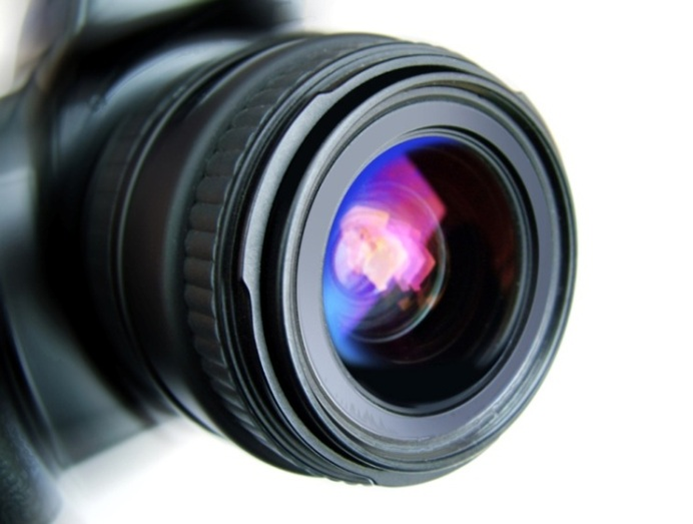
\includegraphics[width=0.8\textwidth]{FigureExample}
\end{center}
\caption{A figure caption}
\label{fig:FigureExample}
\end{figure}  
This was coded using the following:
\begin{verbatim}
\begin{figure}[ht]
\begin{center}
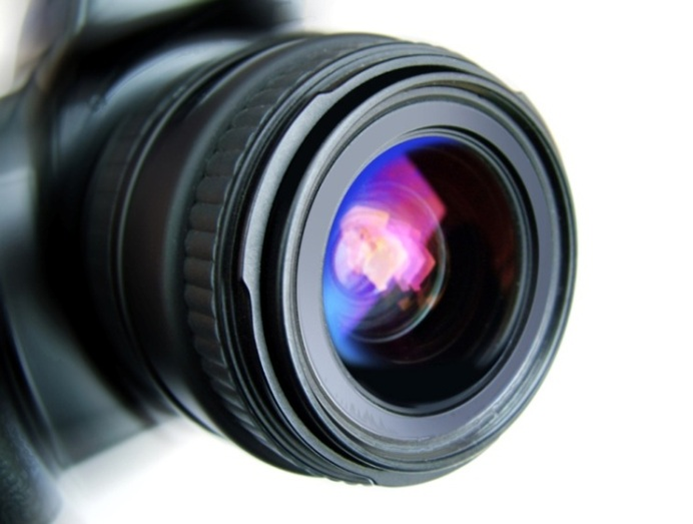
\includegraphics[width=0.8\textwidth]{FigureExample}
\end{center}
\caption{A figure caption}
\label{fig:FigureExample}
\end{figure}  
\end{verbatim}
Note the figure placement options \verb#[ht]# to place the figure as best as possible either (h=) here (at the place where coded) or at the (t=) top of the page. Otherwise it will be placed on the following page. 

If you wish to include sub-figures, that is two or more graphs, phots or diagrams alongside each other with the same main caption then consider using the subfigure package~\cite{bidi-tex_github_organisation_ctan_2005}

\subsection{Tables}
A \LaTeX\ \verb#\table# environment should be used to insert tables, with the table itself generated using the \verb#\tabular# environment.  An example is shown in \reftab{tab:TableExample}.
\begin{table}[ht]
\caption{A table caption}
\begin{center}
\begin{tabular}{l|l|l}
& Heading & Heading \\ \hline
Label & Detail & Detail \\
Label & Detail & Detail \\ \hline
\end{tabular}
\end{center}
\label{tab:TableExample}
\end{table}
The caption should be placed above the table. The coding to achieve this is:
\begin{verbatim}
\begin{table}[ht]
\caption{A table caption}
\begin{center}
\begin{tabular}{l|l|l}
& Heading & Heading \\ \hline
Label & Detail & Detail \\
Label & Detail & Detail \\ \hline
\end{tabular}
\end{center}
\label{tab:TableExample}
\end{table}
\end{verbatim}

\subsection{Equations}
Equations with labels are easily coded in \LaTeX\ using the \verb#equation# and  \verb#\label# environment,
\begin{equation}
A=\pi r^2. \label{eq:circlearea}
\end{equation}
This is coded as
\begin{verbatim}
\begin{equation}
A=\pi r^2. \label{eq:circlearea}
\end{equation}
\end{verbatim}
Remember to punctuate your equation with a period if it ends a sentence. 

Equations should only be labelled if they are cross-referenced later. Use \verb#\[.\]# for an unlabelled equation,
\[
A=\pi r^2.
\]

For a derivations it is often useful to use the \verb#eqnarray# environment. For example, multiplying out a quadratic,
\begin{eqnarray}
y&=&(x-3)(x+4) \nonumber\\
&=& x^{2}+x-12 \label{eq:quadratic}
\end{eqnarray}
with \verb#\nonumber# used to label constituent equations that do not need labelling. This is coded as 
\begin{verbatim}
\begin{eqnarray}
y&=&(x-3)(x+4) \nonumber\\
&=& x^{2}+x-12 \label{eq:quadraticarray}
\end{eqnarray}
\end{verbatim}

\subsection{Referring to captions for figures, tables etc.}
We can reference figures, tables and equations using supplied \verb#\refFig#, \verb#\reffig#, \linebreak\verb#\refTab#, \verb#\reftab#, \verb#\refEqn# or \verb#\refeqn# according to what we are referencing, and whether we are doing so at the start of a sentence or not. Here are some examples:
\begin{itemize}
\item \refTab{tab:TableExample} at start of a sentence
\begin{verbatim}
\refTab{tab:TableExample} at start of a sentence 
\end{verbatim}
\item Within sentence reference to \reftab{tab:TableExample} 
\begin{verbatim}
\item Within sentence reference to \reftab{tab:TableExample} 
\end{verbatim}
\item \refEqn{eq:quadratic} at start of a sentence
\begin{verbatim}
 \refEqn{eq:quadratic} at start of a sentence
\end{verbatim}
\item Within sentence reference to \refeqn{eq:quadratic} 
\begin{verbatim}
\item Within sentence reference to \refeqn{eq:quadratic} 
\end{verbatim}
\end{itemize}

\subsection{Updating Tables of Contents, Lists of Figures and Labels}
The information for contents, figures, tables and labels and cross-referencing for \LaTeX\ are enabled using various files: \verb#.toc# (table of contents), \verb#.lof# (list of figures), \verb#.lot# (list of tables)\verb#.aux# file. e.g., e.g., for this \LaTeX\ file \verb#LaTeX_Thesis_Template.toc#, \verb#LaTeX_Thesis_Template.lof#, \verb#LaTeX_Thesis_Template.lot# and \linebreak \verb#LaTeX_Thesis_Template.aux# are created. The labels, captions etc  are written to these files when a command such as \verb#\chapter# or \verb#\label# when processing the \LaTeX\ file (e.g., when running \verb#pdflatex#).   The labels, chapter names etc. are also read from this file to generate the table of contents, list of tables, cross-references. As a result you will need to process the file at least twice to get the table of contents, list of tables and cross-references correctly updated.

Sometimes these files may get corrupted if the labels, chapter names etc are not correctly coded. In this case you will need to remove the \verb#.toc# (table of contents), \verb#.lof# (list of figures), \verb#.lot# (list of tables)\verb#.aux# files. There is often a simple menu option to do this if using \LaTeX\ through a GUI tool such as \verb#TeXworks# for which the drop down {\em File -- Remove Aux Files ...} may be used.

\begin{landscape}
\section{Inserting Landsape Pages}
It is often preferable to use a landscape page to display tables of data, charts or diagrams.  
\begin{figure}[ht]
\begin{center}
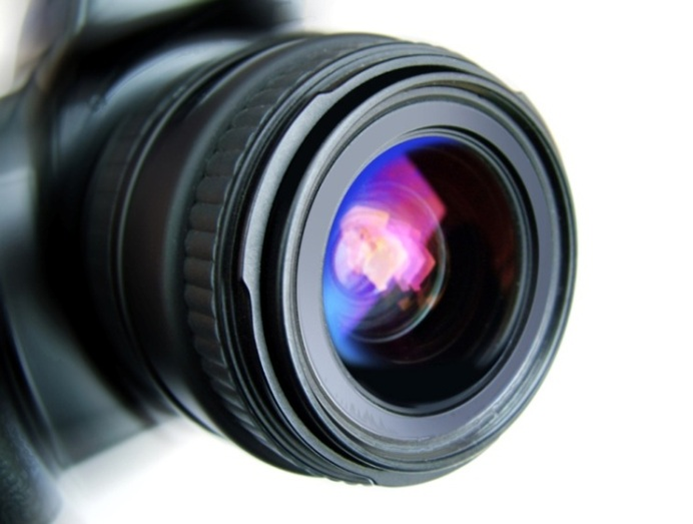
\includegraphics[width=0.8\textwidth]{FigureExample}
\end{center}
\caption{A figure on a rotated page caption}
\label{fig:FigureExampleRotated}
\end{figure} 
This is most easily done by using the \verb#lscape# package~\cite{carlisle_ctan_2020} and placing the \LaTeX\ source for the content to be created with the \verb#landscape# environment. 
\begin{verbatim}
% preamble
% : 
\usepackage{lscape}
% 
\begin{document}
% :
\begin{landscape}
% source for landscape material
\end{landscape}
\end{verbatim}
 
\end{landscape}



\chapter{Referencing}
\label{chap:referencing}
The University specifies that you should use the APA7 Author-Date \cite{cranfield_library_service_apa7_2021} or the Cranfield Numbered \cite{barrington_library_numbered_2016} citation styles as advised by your course director or supervisor. 

\section{Cranfield APA7 Author-Date Referencing}
\label{sec:authordaterefs}
While this author has not used it, the \LaTeX\ bib style apa7~\cite{weiss_ctan_2022} should permit the use of the University's APA7 Author-Date Referencing style~\cite{cranfield_library_service_apa7_2021}.


\section{Cranfield Numbered Referencing} 
\label{sec:CranfieldNumbered}
Ensure the following lines are uncommented in the preamble to the template file. 
\begin{verbatim}
 \usepackage[numbers]{natbib} % for nice referencing
 \makeatletter % Reference list option change to number and period
 \renewcommand\@biblabel[1]{#1.} % from [1] to 1
 \makeatother %
 \setcitestyle{round} % use round citations
 \end{verbatim}
The bibliography style is coded in the \verb#CranfieldNumbered.bst# bibliography style file so this must be stated using the \verb#\bibliographystyle# command
\begin{verbatim}
\bibliographystyle{CranfieldNumbered}
\end{verbatim}
This bibliography style file  has been adapted from that of the standard Vancouver system~\cite{van_der_beek_ctan_2021}.

We now cover a few of the examples from Cranfield Numbered Style~\cite{barrington_library_numbered_2016}. 

\subsection{Books}
\label{sec:NumberedBooks}
\begin{description}
\item[Book with a single author] According to Sommerville~\cite[p.35]{sommerville_software_2007} the most important part of software engineering is…
\item[Book with two authors] Stair and Reynolds \cite[p.65]{stair_principles_2010} suggest…
\item[Book with four or more authors] This was noted by Payne et al. \cite[p.15]{payne_relationship_1995}
\item[Book with an editor] Latest thinking on gender in organizations
suggests… \cite{kumra_oxford_2014}
\item[Chapter of an edited book] Haase~\cite[p.35]{haase_standards_2005} identified...
\item[Chapter of an edited book with organisation as author e.g. handbooks] 
The steel corrosion showed …\cite{asm_international_corrosion_1998}
\item[Book with no author] In order to vote in the UK…\cite{noauthor_whitakers_2011}
\item[Electronic book (eBook) or an online book] The project manager’s role can be defined as… \cite{kerzer_project_2009}
\item[Book accessed via an eReader e.g. Kindle, iPad etc.]
Brodie tried to decipher the \linebreak code~\cite{dennis_secret_2012}\\
\textbf{NOTE: Place eReader type in square brackets at the end of the bibtex title field}
\item[Translated Book] In his discussion about algebraic
topology, Matveev \cite[p.17]{matvev_lectures_2006} considered...\\
\textbf{Translator not yet supported}
\end{description}

\subsection{Journal Articles}
\label{sec:NumberedJournal}
\begin{description}
\item[Journal article with one author] A recent article discussed the
fracture... \cite{hutchinson_fracture_2010}.
\item[Journal article with two or three authors] It was not possible to separate
targets \cite{yang_perceptual_2016}.
\item[Journal article with four or more authors] Langley \etal~\cite{langley_process_2013} identify assumptions\ldots . Note the use of the \verb#\etal# command for the correct, non-italicised, \etal.
\item[Online journal article with DOI] The synthesis of a new polymer of
cadmium(II) \linebreak ethylenediamineazide was determined by \ldots \cite{yang_preparation_2010}. 
\item[Online journal article with URL] The synthesis of a new polymer of
cadmium(II) \linebreak ethylenediamineazide was determined by \ldots \cite{yang_another_2010}.\\\textbf{NOTE: The bibtex style file does not support the \texttt{accessed} attribute so include it in the note field of the bibtex entry.}
\item[Journal article with no author]  TC-32B QT was demonstrated at an
exhibition held in Kent \cite{anon_first_2005}.
\end{description}

\subsection{Conference Papers}
\label{sec:NumberedConference}
\textbf{NOTE:} Use bibtex entry \texttt{incollection}.
\begin{description}
\item[Full conference proceeding] The IEEE \cite[p.59]{noauthor_11_2010} suggests that \ldots
\item[Individual paper] Moon and Koh \cite{moon_aeroacoustic_2003} provide computations \ldots\\
\textbf{NOTE:} Place paper number in the bibtex \texttt{number} field.
\item[Online proceeding or paper] Wessel and Meyer \cite{wessel_assessing_2010} provide a ten step method\ldots
\item[Offshore Technology Conference (OTC) paper] According to Chiasson, Smith and
Steward \cite{chiasson_large_1999} large bore \ldots
\end{description}

\subsection{Internet}
\label{sec:Internet}
\textbf{NOTES:} 
\begin{itemize}
\item The bibtex style file does not support the \texttt{accessed} attribute so include it in the note field of the bibtex entry.
\item If using Zotero then use a \texttt{document} and not a \texttt{web} entry as the \texttt{publisher} field is often used
\end{itemize}
\begin{description}
\item[Web page with an individual author] Bradley \cite{bradley_notitle_2011} states that libraries and \ldots
\item[Web page with an organisation as author] The Natural Hazards Centre \cite{university_of_colorado_boulder_natural_2011} advised
that \ldots
\item[Blog] Julian Borger \cite{borger_afghanistan_2010} claims in `Afghanistan
options are running out' \ldots\\
\textbf{NOTE: add [Blog] to end of title field.}
\item[Wiki] The CILIP ARLG National committee
meeting notes show\ldots \cite{barefoot_october_2012}
\textbf{NOTE: add [Wiki] to end of title field.}
\end{description}

\subsection{Thesis or dissertation}
\label{sec:thesis}
\begin{description}
\item[Print thesis or dissertation] An examination of Forth’s \cite{forth_morphological_1989}
research shows that…
\item[Online thesis or dissertation] Tatham \cite{tatham_confidence_2010} identifies three areas
undergoing notable change…\\
\textbf{NOTE: use of question mark in thesis title is not presently detected in bibtex style file.}
\end{description}


\subsection{Course materials}
\label{sec:course}
\begin{description}
\item[Lecture or seminar] The lecture provoked much debate~\cite{johnson_peat_2012}
\item[Lecturers’ notes on Virtual Learning Environment \eg\ Canvas] As illustrated in the course materials~\cite{forth_analysis_2012}
\item[Course Virtual Learning Environment discussion forum] The debate during the lecture continued in the discussion forum. Hirst \cite{hurst_are_2012} was
particularly vociferous.
\end{description}

\subsection{Official Publications}
\label{sec:officialPubs}
\textbf{Note:} These have not been tested yet but can probably be achieved with a bibtex \verb#misc# entry.
\begin{description}
\item[UK Statute (Act of Parliament)] 
\item[House of Commons or House of Lords Paper]
\item[House of Commons or House of Lords Bill]
\item[Statutory Instruments (SIs)]
\item[Hansard Debate]
\item[Command Paper (Green or White Paper)]
\item[European Directive]
\end{description}

\subsection{Reports}
\label{sec:Reports}
\begin{description}
\item[Report] An analysis of China’s investment in companies in different countries has shown... \cite{wolf_chinas_2011}.
\item[Online report] The effect was… \cite{curry_-flight_1989}.\\
\textbf{Note:} Presently unable to get colon (:) between report number and report title.
\item[Online industry or market research report] Media trends in the UK…\cite{marketline_media_2013}
\item[Online company or annual report] Despite economic uncertainty the
company’s profits did increase \cite{rolls-royce_group_plc_annual_2011}.
\item[Online company or financial report or data source] Rolls-Royce plc turnover has dramatically
reduced in 2009-2010 \cite{bureau_van_dijk_rolls-royce_2010}.
\end{description}


\subsection{Case Studies}
\textbf{Note:} These have not been tested yet but can probably be achieved with a bibtex \verb#misc# entry.

\subsection{Working Papers}
\textbf{Note:} These have not been tested yet but can probably be achieved with a bibtex \verb#misc# entry.

\subsection{Newspapers}
\label{Sec:Newspapers}
\textbf{Note:} 
\begin{itemize}
\item Use bibtex \verb#misc# type, zotero 
\item If needed place edition (\eg Evening Ed.) in the Newspaper (bibtex \verb#journal# field) title.
\end{itemize}
\begin{description}
\item[Printed newspaper article] A blast at an atomic weapons factory was
met with denials by Iran \cite{frenkel_europe_nodate}.\\
\textbf{Note:} Use bibtex \texttt{misc} type, omit date from \texttt{year} field and place date in \texttt{note} field. 
\item[Article from an online newspaper]  Rayner \cite{rayner_combat_2011} reports that The Royal British Legion Centre for Blast Injury Studies is
to design…
\end{description}


\subsection{Standards, patents, protocols and datasheets}
\label{sec:standards}
\textbf{Note:} 
\begin{itemize}
\item Use bibtex \texttt{report} item
\item Presently unable to get colon (:) between report number and report title.
\end{itemize}
\begin{description}
\item[Standard] In projects "specification, schedule and
cost always have to be bounded to ensure
ongoing viability" \cite{british_standards_institution_project_2010}.
\item[Online standard from a database] Some standards provide guidelines for effective project management \cite{british_standards_institution_project_2010}.
\item[Patent] The method of assembly... \cite{hodge_rear_2008}
\item[Joint Service Publication or protocol] The MOD has a simple definition of knowledge \cite{great_britain_ministry_of_defence_retaining_2011}.\\
\textbf{Note:} As the actual url is not available, put the availability and accessed data in the bibtex \texttt{note} field.
\item[Datasheet \eg ESDU] The buckling of the panel… \cite{esdu_elastic_2008}.
\end{description}

\subsection{Datasets and software}
\label{sec:datasets}
\begin{itemize}
\item Use bibtex \texttt{misc} type.
\item Include version number in parenthesis in the \texttt{title} field.
\end{itemize}
\begin{description}
\item[Dataset] Data from Partridge \cite{partridge_spectra_2014} showed \ldots
\item[Software] Plone is an example of this sort of use
of an open source content management
system~\cite{plone_foundation_plone_2016}.
\end{description}

\subsection{Audio visual materials}
\textbf{Note:} These have not been tested yet but can probably be achieved with a bibtex \verb#misc# entry.

\subsection{Images}
\label{sec:images}
\textbf{Notes:} 
\begin{itemize}
\item Use \texttt{misc} type
\item For items available online   so include the \texttt{accessed} attribute in the \texttt{note} field of the bibtex entry.
\end{itemize}
\begin{description}
\item[Illustration, figure, diagram, logo or table] The estimated sales forecast is shown in \reffig{fig:sales}.
\begin{figure}[ht]
\begin{center}
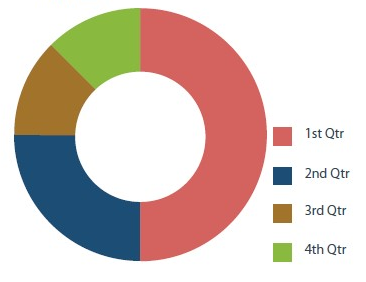
\includegraphics[width=0.6\textwidth]{Sales}
\end{center}
\caption{Estimated Sales Forecast~\cite[p.4]{wisker_good_2012}}
\label{fig:sales}
\end{figure}
\item[Embedded illustration, cartoon, diagram, etc.] The pressure on the housing market… \cite{wood_cartoon_2014}.\\
\textbf{Note:} Include the \texttt{[medium]} , here a \texttt{[cartoon]} at the start of the bibtex title field.
\item[Ordnance Survey map] P.O. equates to Post Office \cite{ordnance_survey_oxford_1994}.\\
\textbf{Note:} 
\begin{itemize}
\item Use the \texttt{title} field to add the map number and scale.
\item Use the \texttt{note} field to add the map series.
\end{itemize}
\item[Online map] There are many farms in the area \cite{ordnance_survey_peak_2010}.\\
\textbf{Note:} The bibtex style file does not support the \texttt{accessed} attribute so include it in the note field of the bibtex entry.
\item[Painting or drawing] \textbf{Note:} This has not been tested yet but can probably be achieved with a bibtex \verb#misc# entry.
\item[Painting or drawing online] Groves’ {\em Carrot on a stick} \cite{groves_carrot_2007} is playing with colours. 
\item[Photograph – print or slide] 
Sublime lighting captures the atmosphere
wonderfully \cite{collins_pictures_2010}\\
\textbf{Note:} I uses a \texttt{book} entry here.
\item[Photograph online or in an online collection \eg Flickr, Instagram] An abundance of movement is
captured \cite{rush_running_1997}.
\end{description}


\subsection{Personal communications}
\textbf{Notes:}\\
\begin{itemize}
\item Use \texttt{misc} type
\item If dates are not fully listed then place them in the \texttt{note} field.
\end{itemize}
\begin{description}
\item[Email or letter] The details of the organisational structure
were outlined \cite{godfrey_restructure_nodate}.
\item[Conversation] It was felt the organisational culture
changed when the new CEO arrived \cite{williams_conversation_nodate}.
\item[Interview, survey or questionnaire] The theory was dismissed as
nothing new \cite{benson_should_nodate}.
\end{description}



\chapter[Dealing with long chapter names]{Dealing with chapters whose 
chapter name is ridiculously long and so spoiling formatting}
Apart from new chapter pages, the style file automatically uses the current chapter and section names for the left and right headers of the pages of the main body. This can cause problems if the chapter or section names are tool long. To cope with this, when you define the new chapter, also define a shortened chapter name in square brackets as we have for this chapter,
\begin{verbatim}
\chapter[Dealing with long chapter names]{Dealing with chapters whose 
chapter name is ridiculously long and so spoiling formatting}
\end{verbatim}
\refSec{sec:longSection} shows how to do this for sections. 

Note that the short chapter and section names are also used in the table of contents so try to avoid long names if possible.

\newpage
\section[Dealing with long section names]{Dealing with sections whose 
section name is ridiculously long and so spoil formatting}
\label{sec:longSection}
For long section names it's advisable to provide a short section name
\begin{verbatim}
\section[Dealing with long section names]{Dealing with sections whose 
section name is ridiculously long and so spoil formatting}
\end{verbatim}


\chapter{More Topics}
This is a sample of thesis text. This is a sample of thesis text. This is a 
sample of thesis text. This is a sample of thesis text. This is a sample of
thesis text.

This is a sample of thesis text. This is a sample of thesis text. This is a 
sample of thesis text. This is a sample of thesis text. This is a sample of
thesis text.


\chapter{Final Topic}
This is a sample of thesis text. This is a sample of thesis text. This is a 
sample of thesis text. This is a sample of thesis text. This is a sample of
thesis text.

This is a sample of thesis text. This is a sample of thesis text. This is a 
sample of thesis text. This is a sample of thesis text. This is a sample of
thesis text.


\chapter{Conclusions}
This is a sample of thesis text. This is a sample of thesis text. This is a 
sample of thesis text. This is a sample of thesis text. This is a sample of
thesis text.

This is a sample of thesis text. This is a sample of thesis text. This is a 
sample of thesis text. This is a sample of thesis text. This is a sample of
thesis text.


%% Back matter
%
% This is where we include references and appendices

\bibliographystyle{CranfieldNumbered}
\bibliography{LaTeX,CUCitations}


\appendix
\chapter{Ethical Approval Letter}
Insert your Ethical Approval Letter as the first appendix.

\chapter{Extra Data}
This is a sample of thesis text. This is a sample of thesis text. This is a 
sample of thesis text. This is a sample of thesis text. This is a sample of
thesis text.

This is a sample of thesis text. This is a sample of thesis text. This is a 
sample of thesis text. This is a sample of thesis text. This is a sample of
thesis text.





\end{document}

